\section{Props with Exponentiation and Generalized Control}
%
\label{Sect:Hierarchical}

Hierarchical quantum circuits build upon the prop formalism by introducing two new connectives, namely $( \odot )$ and $( \exparr )$.
The $( \odot )$ connective can be thought of as an abstraction of generalized control, and the $( \exparr )$ connective can be thought of as an abstraction of circuit exponentiation.
As outlined in the previous section, the $( \odot )$ connective should be associative, though few assumptions can be made about the $( \exparr )$ connective.
In particular, neither $( \odot )$ nor $( \exparr )$ are functorial in general.
This means that unlike a controlled prop, it does not suffice to simply complete a standard prop under the application of two functors.
Instead, the hierarchical language will be constructed in levels, with the lowest level corresponding to a standard prop.

The basic idea of this construction is that given a free prop $P( \Sigma )$, the powers and generalized controls can be freely constructed as purely syntactic objects.
Since circuits in $P( \Sigma )$ are equal up to diagram isomorphism, then their exponentiated and controlled forms will also be equal up to isomorphism of their subcircuit constituents.
These syntactic objects are then combined with the gates in $\Sigma$ to generate a strictly larger prop containing $P( \Sigma )$, and the process repeats.
More formally, the construction proceeds as follows.

\begin{figure}[t]
    % --------------------------------------------------------
    \begin{subfigure}[b]{0.17\textwidth}
        \centering
        \scalebox{0.65}{\circimg{tikz-cache/notation__power.pdf}}
        \caption{$U \exparr \alpha$.}
        \label{Fig:Extended:Power}
    \end{subfigure}
    % --------------------------------------------------------
    \begin{subfigure}[b]{0.17\textwidth}
        \centering
        \scalebox{0.65}{\circimg{tikz-cache/notation__bictrl.pdf}}
        \caption{$U \odot V$.}
        \label{Fig:Extended:BiCtrl}
    \end{subfigure}
    % --------------------------------------------------------
    \begin{subfigure}[b]{0.22\textwidth}
        \centering
        \scalebox{0.65}{\circimg{tikz-cache/notation__trictrl.pdf}}
        \caption{$U \odot V \odot W$.}
        \label{Fig:Extended:TriCtrl}
    \end{subfigure}
    % --------------------------------------------------------
    \begin{subfigure}[b]{0.39\textwidth}
        \centering
        \scalebox{0.65}{\circimg{tikz-cache/notation__example.pdf}}
        \caption{$U \in \CatHQC[2]( 3, 3 ) \setminus \CatHQC[1]( 3, 3 )$.}
    \end{subfigure}
    % --------------------------------------------------------
    \caption{A graphical language for the morphisms in $\CatHQC$. In these diagrams we assume that $U: n \to n$, $V: m \to m$, and $W: \ell \to \ell$.}
    \label{Fig:Extended}
\end{figure}

\vspace{1em}
\noindent
\textbf{Exponentiation}.
Let $\mathcal{C}$ be a prop category.
If $U \in \Mor( \mathcal{C} )$ and $\alpha \in \mathbb{R}$, then there should be a unique term $U \exparr \alpha$ which is thought of as exponentiating $U$ by $\alpha$.
Since we do not require exponentiation to satisfy any further properties, then $\Power( \mathcal{C} ) := \Mor( \mathcal{C} ) \times \mathbb{R}$.
We write $U \exparr \alpha$ for an element $( U, \alpha ) \in \Power( \mathcal{C} )$.
Of course, $\dom( U \exparr \alpha ) = \dom( U )$ and $\cod( U \exparr \alpha ) = \cod( U )$.
A term of the form $U \exparr \alpha$ is denoted by raising $U$ to the power of $\alpha$, as depicted in \cref{Fig:Extended:Power}.

\vspace{1em}
\noindent
\textbf{Generalized Controls}.
Let $\mathcal{C}$ be a prop category.
Since $( \odot )$ is known to be associative, then it suffices to generate the free monoid $\Mor( \mathcal{C} )^*$ on $\Mor( \mathcal{C} )$.
We write $U_1 \odot U_2 \odot \cdots \odot U_n$ for an element $( U_1, U_2, \ldots, U_n ) \in \Mor( \mathcal{C} )^*$.
Of course, only terms of length two or more correspond to valid generalized controls in the circuit language.
We write $\Tower( \mathcal{C} ) := \{ T \in \Mor( \mathcal{C} )^* : |T| \ge 2 \}$.
If $T \in \Tower( \mathcal{C} )$, then $\dom( T ) = \sum_{j=1}^n \dom( T_j )$ and $\cod( T ) = \sum_{j=1}^n \cod( T_j )$ where $n = |T|$.
An $n$-ary $(\odot)$-product is illustrated by a vertical wire joining the $n$ factors, as in \cref{Fig:Extended:BiCtrl} and \cref{Fig:Extended:TriCtrl}.

\vspace{1em}
\noindent
\textbf{Constructing the Hierarchy}.
The construction begins with a primitive gate set $\Sigma_{\mathbf{Prim}}$.
In the case of this paper,
$\Sigma_{\mathbf{Prim}} = \{
        \scalebox{0.65}{\circimg{tikz-cache/dagger__term1.pdf}},
        \scalebox{0.65}{\circimg{tikz-cache/dagger__term2.pdf}},
        \scalebox{0.65}{\circimg{tikz-cache/dagger__term3.pdf}},
        \scalebox{0.65}{\circimg{tikz-cache/dagger__term4.pdf}},
        \scalebox{0.65}{\circimg{tikz-cache/dagger__term5.pdf}},
        \scalebox{0.65}{\circimg{tikz-cache/dagger__term8.pdf}}
\}$.
This gives rise to a free prop $\CatHQC[0] = P( \Sigma_{\CatHQC}^0 )$ where $\Sigma_{\CatHQC}^0 = \Sigma_{\mathbf{Prim}}$.
The construction then proceeds inductively as follows.
For each $n \in \mathbb{N}$, define a signature $\Sigma_{\CatHQC}^{n+1} = \Sigma_{\CatHQC}^n \cup \Tower( \CatHQC[n] ) \cup \Power( \CatHQC[n] )$ and a prop category $\CatHQC[n+1] = P( \Sigma_{\CatHQC}^{n+1} )$.
Since $\Sigma_{\CatHQC}^n \subseteq \Sigma_{\CatHQC}^{n+1}$, then this construction can be summarized by the following diagram.
\begin{center}
    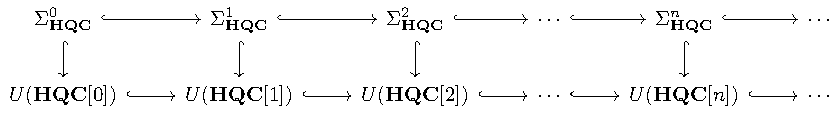
\includegraphics{tikz/language.pdf}
\end{center}

Since $\Mor( \CatHQC[n] ) \subseteq \Mor( \CatHQC[n+1] )$, then there is an identification of monoid generators such that $\Tower( \CatHQC[n] ) \le \Tower( \CatHQC[n+1] )$ in the sense of submonoids.
We will assume this identification, such that if $T \in \Tower( \CatHQC[n] )$ with $k = |T|$ and $S \in \Tower( \CatHQC[n+1] )$, then $T \odot S = T_1 \odot ( T_2 \odot ( \cdots \odot ( T_k \odot S ) ) )$.
The categorical colimit of this construction is denoted $\CatHQC$, so that $\CatHQC = P( \Sigma_{\CatHQC} )$ where $\Sigma_{\CatHQC} = \bigcup_{n=0}^\infty \Sigma_{\CatHQC}^n$.
The following lemmas characterize how to map freely out of $\CatHQC$ where $\sqcup$ denotes the disjoint union of sets.

\begin{lemma}
    \label{Lem:FuncDefFam}
    Let $\Sigma_0^* = \Sigma_{\CatHQC}^0$ and $\Sigma_{n+1}^* = \Sigma_{\CatHQC}^{n+1} \setminus \Sigma_{\CatHQC}^n$ for each $n \in \mathbb{N}$.
    If $\left\{ \tau_n: \Sigma^*_{n} \to U( \mathcal{C} ) \right\}_{n=0}^{\infty}$ is a family of prop signature morphisms, then there exists a unique prop functor $F: \CatHQC \to \mathcal{C}$ such that $F( g ) = \tau_n( g )$ for each $n \in \mathbb{N}$ and $g \in \Sigma_n^*$.
\end{lemma}

\begin{lemma}
    \label{Lem:FuncDefPart}
    $
        \Sigma_{\CatHQC}
        =
        \Sigma_{\mathbf{Prim}}
        \sqcup \Sigma_{\mathbf{Ctrl}}
        \sqcup
        \Sigma_{\mathbf{Pow}}
    $
    where
    $
        \Sigma_{\mathbf{Ctrl}}
        =
        \{ U \odot V : U, V \in \Mor( \CatHQC ) \}
    $
    and
    $
        \Sigma_{\mathbf{Pow}}
        =
        \{
            U \exparr \alpha
            :
            U \in \Mor( \CatHQC )
            \text{ and }
            \alpha \in \mathbb{R}
        \}
    $.
\end{lemma}

It should come as no surprise that the standard semantic interpretation for $\CatHQC$ is defined in terms of the generalized controls and exponentiation in $\CatUnitary$.
It follows from \cref{Lem:FuncDefFam} that the following set of equations defines a unique prop functor $\sem{-}_H: \CatHQC \to \CatUnitary$.
Note that this is well-defined since $( \odot )$ is also associative for $\CatUnitary$ by \cref{Thm:ControlAssoc}.
\begin{align*}
    s_0\left( \scalebox{0.65}{\circimg{tikz-cache/dagger__term1.pdf}} \right)
    &=
    Z
    %\scalebox{0.65}{$\begin{bmatrix}
    %    1 & 0 \\
    %    0 & -1
    %\end{bmatrix}$}
    &
    s_0\left( \scalebox{0.65}{\circimg{tikz-cache/dagger__term2.pdf}} \right)
    &=
    -Z
    %\scalebox{0.65}{$\begin{bmatrix}
    %    -1 & 0 \\
    %    0 & 1
    %\end{bmatrix}$}
    &
    s_0\left( \scalebox{0.65}{\circimg{tikz-cache/dagger__term3.pdf}} \right)
    &=
    X
    %\scalebox{0.65}{$\begin{bmatrix}
    %    0 & 1 \\
    %    1 & 0
    %\end{bmatrix}$}
    &
    s_0\left( \scalebox{0.65}{\circimg{tikz-cache/dagger__term4.pdf}} \right)
    &=
    -X
    %\scalebox{0.65}{$\begin{bmatrix}
    %    0 & -1 \\
    %    -1 & 0
    %\end{bmatrix}$}
    &
    s_0\left( \scalebox{0.65}{\circimg{tikz-cache/dagger__term8.pdf}} \right)
    &= -1
\end{align*}
\vspace{-2em}
\begin{align*}
    s_0\left( \scalebox{0.65}{\circimg{tikz-cache/dagger__term5.pdf}} \right)
    &=
    H
    %\scalebox{0.65}{$\frac{1}{\sqrt{2}}\begin{bmatrix}
    %    1 & 1 \\
    %    1 & -1
    %\end{bmatrix}$}
    &
    %s_{n+1}\left( \bigodot_{j=1}^k U_j \right) 
    %&=
    %\bigodot_{j=1}^k s_n( U_j )
    s_{n+1}( U_1 \odot \cdots \odot U_k )
    &=
    s_n( U_1 ) \odot \cdots \odot s_n( U_k )
    &
    s_{n+1}\left( U \exparr \alpha \right)
    &=
    s_n( U )^\alpha
\end{align*}
The following set of equations are also well-defined by \cref{Lem:FuncDefPart}, and define a unique prop functor $\dagger: \CatHQC \to \CatHQC^\text{op}$ which sends each circuit in $\CatHQC$ to its syntactic adjoint.
\begin{align*}
    d \left( \scalebox{0.65}{\circimg{tikz-cache/dagger__term1.pdf}} \right)
        &= \scalebox{0.65}{\circimg{tikz-cache/dagger__term1.pdf}}
    &
    d \left( \scalebox{0.65}{\circimg{tikz-cache/dagger__term2.pdf}} \right)
        &= \scalebox{0.65}{\circimg{tikz-cache/dagger__term2.pdf}}
    &
    d \left( \scalebox{0.65}{\circimg{tikz-cache/dagger__term3.pdf}} \right)
        &= \scalebox{0.65}{\circimg{tikz-cache/dagger__term3.pdf}}
    &
    d \left( \scalebox{0.65}{\circimg{tikz-cache/dagger__term4.pdf}} \right)
        &= \scalebox{0.65}{\circimg{tikz-cache/dagger__term4.pdf}}
    &
    d \left( \scalebox{0.65}{\circimg{tikz-cache/dagger__term5.pdf}} \right)
        &= \scalebox{0.65}{\circimg{tikz-cache/dagger__term5.pdf}}
\end{align*}
\vspace{-2em}
\begin{align*}
    d \left( \scalebox{0.65}{\circimg{tikz-cache/dagger__term8.pdf}} \right)
        &= \scalebox{0.65}{\circimg{tikz-cache/dagger__term8.pdf}}
    &
    d \left( \scalebox{0.65}{\circimg{tikz-cache/dagger__term7_lhs.pdf}} \right)
        &= \scalebox{0.65}{\circimg{tikz-cache/dagger__term7_rhs.pdf}}
    &
    d \left( \scalebox{0.65}{\circimg{tikz-cache/dagger__term6_lhs.pdf}} \right)
        &= \scalebox{0.65}{\circimg{tikz-cache/dagger__term6_rhs.pdf}}
\end{align*}

\begin{theorem}
    \label{Thm:DagSem}
    If $U \in \Mor( \CatHQC )$, then $\sem{U^\dagger}_H = \sem{U}_H^\dagger$.
\end{theorem}

Given the syntactic adjoint map $( \dagger )$, it is then possible to define syntactic diagonalization.
Fix some $n \in \mathbb{N}$ which will denote the number of wires in these circuits.
Then for each $x \in \{ 0, 1 \}^n$ and $\alpha \in \mathbb{R}$, there exists a circuit $\lambda( x, \alpha ) \in \CatHQC( n, n )$ such that $\sem{ \lambda( x, \alpha ) }_H = \exp( i H )$ where $H = \alpha \bigotimes_{j=0}^{n-1} \ket{x_j} \bra{x_j}$.
Moreover, $\lambda( x, \alpha )$ can be constructed entirely from NOT-gates and global phase gates with zero or more $Z$-controls (see~\cref{App:DiagGate}).
A circuit $\Lambda$ is in \emph{diagonal form} if there exists a bijection $f: \{ 1, 2, \ldots, 2^n \} \to \{ 0, 1 \}^n$ and function $\alpha: \{ 1, 2, \ldots, 2^n \} \to ( -\pi, \pi ]$ such that $\Lambda = \lambda( f( 1 ), \alpha( 1 ) ) \circ \cdots \circ \lambda( f( 2^n ), \alpha( 2^n ) )$.
Then a syntactic diagonalization of $U \in \CatHQC( n, n )$ is a choice of diagonal form $\Lambda \in \CatHQC( n, n )$ and $P \in \CatHQC( n, n )$ such that $\sem{U}_H = \sem{P^\dagger \circ \Lambda \circ P}_H$.

\subsection{A Sound Equational Theory with Unitary Controls}
%
\label{Sect:Background:Theory}

\begin{figure}[t]
    \begin{framed}
        \textbf{Collection 1: Ordinary Circuit Relations}
        \vspace{-1em}
        \begin{align*}
            \scalebox{0.65}{\circimg{tikz-cache/hqc__eqn8_lhs.pdf}}
            &\overset{\HqcHDef}{=}
            \scalebox{0.65}{\circimg{tikz-cache/hqc__eqn8_rhs.pdf}}
            & % -------------------------------------------------------
            \scalebox{0.65}{\circimg{tikz-cache/hqc__eqn10_lhs.pdf}}
            &\overset{\HqcTargDef}{=}
            \scalebox{0.65}{\circimg{tikz-cache/hqc__eqn10_rhs.pdf}}
            & % -------------------------------------------------------
            \scalebox{0.65}{\circimg{tikz-cache/hqc__eqn11_lhs.pdf}}
            &\overset{\HqcOPhaseDef}{=}
            \scalebox{0.65}{\circimg{tikz-cache/hqc__eqn11_rhs.pdf}}
        \end{align*}
        \vspace{-2.5em}
        \begin{align*}
            \scalebox{0.65}{\circimg{tikz-cache/hqc__eqn12_lhs.pdf}}
            &\overset{\HqcTargMDef}{=}
            \scalebox{0.65}{\circimg{tikz-cache/hqc__eqn12_rhs.pdf}}
            & % -------------------------------------------------------
            \scalebox{0.65}{\circimg{tikz-cache/proofs__decode_q3_lhs.pdf}}
            &\overset{\HqcSwapDef}{=}
            \scalebox{0.65}{\circimg{tikz-cache/proofs__decode_q3_mid.pdf}}
            & % -------------------------------------------------------
            \scalebox{0.65}{\circimg{tikz-cache/hqc__euler_lhs.pdf}}
            &\overset{\HqcEuler}{=}
            \scalebox{0.65}{\circimg{tikz-cache/hqc__euler_rhs.pdf}}
            & % -------------------------------------------------------
            \scalebox{0.65}{\circimg{tikz-cache/hqc__eqn7_lhs.pdf}}
            &\overset{\HqcPOrd}{=}
            \scalebox{0.65}{\circimg{tikz-cache/cqc__eqn1_rhs.pdf}}
        \end{align*}
        
        \textbf{Collection 2: Generalized Control Relations}
        \vspace{-0.5em}
        \begin{align*}
            \scalebox{0.65}{\circimg{tikz-cache/hqc__eqn1_lhs.pdf}}
            &\overset{\HqcCtrlId}{=}
            \scalebox{0.65}{\circimg{tikz-cache/hqc__eqn1_rhs.pdf}}
            & % -------------------------------------------------------
            \scalebox{0.65}{\circimg{tikz-cache/hqc__eqn2_lhs.pdf}}
            &\overset{\HqcCtrlComp}{=}
            \scalebox{0.65}{\circimg{tikz-cache/hqc__eqn2_rhs.pdf}}
            & % -------------------------------------------------------
            \scalebox{0.65}{\circimg{tikz-cache/hqc__eqn3_lhs.pdf}}
            &\overset{\HqcCtrlSwap}{=}
            \scalebox{0.65}{\circimg{tikz-cache/hqc__eqn3_rhs.pdf}}
            & % -------------------------------------------------------
            \scalebox{0.65}{\circimg{tikz-cache/hqc__eqn18_lhs.pdf}}
            &\overset{\HqcFreePhase}{=}
            \scalebox{0.65}{\circimg{tikz-cache/hqc__eqn18_rhs.pdf}}
        \end{align*}
        \vspace{-1.5em}
        \begin{align*}
            \scalebox{0.65}{\circimg{tikz-cache/hqc__eqn14_lhs.pdf}}
            &\overset{\HqcCtrlDag}{=}
            \scalebox{0.65}{\circimg{tikz-cache/hqc__eqn14_rhs.pdf}}
            & % -------------------------------------------------------
            \scalebox{0.65}{\circimg{tikz-cache/hqc__eqn15_lhs.pdf}}
            &\overset{\HqcCtrlPair}{=}
            \scalebox{0.65}{\circimg{tikz-cache/hqc__eqn15_rhs.pdf}}
            & % -------------------------------------------------------
            \scalebox{0.65}{\circimg{tikz-cache/hqc__eqn22_lhs.pdf}}
            &\overset{\HqcCtrlExpand}{=}
            \scalebox{0.65}{\circimg{tikz-cache/hqc__eqn22_rhs.pdf}}
        \end{align*}
        \vspace{-1.5em}
        \begin{align*}
            \scalebox{0.65}{\circimg{tikz-cache/hqc__eqn23_lhs.pdf}}
            &\overset{\HqcCtrlMerge}{=}
            \scalebox{0.65}{\circimg{tikz-cache/hqc__eqn23_rhs.pdf}}
        \end{align*}
        
        \textbf{Collection 3: Generalized Exponential Relations}
        \vspace{-1em}
        \begin{align*}
            \scalebox{0.65}{\circimg{tikz-cache/hqc__eqn9_lhs.pdf}}
            &\overset{\HqcPowZero}{=}
            \scalebox{0.65}{\circimg{tikz-cache/hqc__eqn9_rhs.pdf}}
            & % -------------------------------------------------------
            \scalebox{0.65}{\circimg{tikz-cache/hqc__eqn4_lhs.pdf}}
            &\overset{\HqcPowId}{=}
            \scalebox{0.65}{\circimg{tikz-cache/hqc__eqn4_rhs.pdf}}
            & % -------------------------------------------------------
            \scalebox{0.65}{\circimg{tikz-cache/hqc__eqn5_lhs.pdf}}
            &\overset{\HqcPowAdd}{=}
            \scalebox{0.65}{\circimg{tikz-cache/hqc__eqn5_rhs.pdf}}
            & % -------------------------------------------------------
            \scalebox{0.65}{\circimg{tikz-cache/hqc__eqn24_lhs.pdf}}
            &\overset{\HqcPowIdem}{=}
            \scalebox{0.65}{\circimg{tikz-cache/hqc__eqn24_rhs.pdf}}
        \end{align*}
        \vspace{-2.5em}
        \begin{align*}
            \scalebox{0.65}{\circimg{tikz-cache/hqc__eqn19_lhs.pdf}}
            &\overset{\HqcPowDag}{=}
            \scalebox{0.65}{\circimg{tikz-cache/hqc__eqn19_rhs.pdf}}
            & % -------------------------------------------------------
            \scalebox{0.65}{\circimg{tikz-cache/hqc__eqn21_lhs.pdf}}
            &\overset{\HqcPowExpand}{=}
            \scalebox{0.65}{\circimg{tikz-cache/hqc__eqn21_rhs.pdf}}
        \end{align*}
        
        \textbf{Collection 4: Congruence Relations (Inductively Defined)}
        \vspace{-1em}
        \begin{equation*}
            \scalebox{0.65}{\circimg{tikz-cache/hqc__equiv_lhs.pdf}}
            \approx_E
            \scalebox{0.65}{\circimg{tikz-cache/hqc__equiv_rhs.pdf}}
            %
            \qquad\Rightarrow\qquad
            %
            \scalebox{0.65}{\circimg{tikz-cache/hqc__eqn20_lhs.pdf}}
            \overset{\HqcPowCong}{=}
            \scalebox{0.65}{\circimg{tikz-cache/hqc__eqn20_rhs.pdf}}
            %
            \qquad\text{and}\qquad
            %
            \scalebox{0.65}{\circimg{tikz-cache/hqc__eqn13_lhs.pdf}}
            \overset{\HQCCtrlCong}{=}
            \scalebox{0.65}{\circimg{tikz-cache/hqc__eqn13_rhs.pdf}}
        \end{equation*}
        
        \vspace{-1.5em}
    \end{framed}

    \caption{An equational theory for the category of hierarchical quantum circuits in which $\alpha, \beta, \theta_1, \theta_2 \in \mathbb{R}$, $( \phi_0\pi, \phi_1\pi, \phi_2\pi, \phi_3\pi ) = \mathsf{Euler}( \theta_1\pi, \theta_2\pi )$, $x \in \{ 0, 1 \}^n$, $y \in \{ 0, 1 \}^m$, and $\rho, \gamma \in (-\pi, \pi]$.
    The circuits $\Lambda$ and $\Gamma$ are prefixes of diagonal forms such that a lambda generator with binary string $x$ does not appear in $\Lambda$.}
    \label{Fig:HQCEqnTheory}
\end{figure}

The equational theory $E$ for hierarchical quantum circuits can be found in~\cref{Fig:HQCEqnTheory}.
Some care must be taken when defining this equational theory, since \cref{Fig:HQCEqnTheory} also includes congruence relations, such as $( V \approx_E W ) \Rightarrow ( U \odot V \approx_E U \odot W )$.
To avoid cyclic reasoning, $E$ must be defined inductively.
First, let $E_0$ denote the set of relations described by $\HqcHDef$ through $\HqcPowExpand$.
Then for each $n \in \mathbb{N}$, define $E_{n+1}$ as follows.
\begin{align*}
    E_{n+1}
    =
    E_n
    &\cup
    \{ ( V \exparr \alpha, W \exparr \alpha ) : \alpha \in \mathbb{R} \text{ and } V \approx_{E_n} W \}
    &
    (\text{see \HqcPowCong})
    \\
    &\cup
    \{ ( U \odot V, U \odot W ) : U \in \Mor( \CatHQC ) \text{ and } V \approx_{E_n} W \}
    &
    (\text{see \HQCCtrlCong})
\end{align*}
Then $E = \bigcup_{n=0}^\infty E_n$, so that $U \approx_E V$ if and only if there exists some $n \in \mathbb{N}$ such that $U \approx_{E_n} V$.
It follows from $E(1-4)$ that all of $\CatHQC / E$ can be generated using only two of the three gates in
$\{
        \scalebox{0.65}{\circimg{tikz-cache/dagger__term1.pdf}},
        \scalebox{0.65}{\circimg{tikz-cache/dagger__term3.pdf}},
        \scalebox{0.65}{\circimg{tikz-cache/dagger__term5.pdf}}
\}$ together with
$\{
    \;\scalebox{0.65}{\circimg{tikz-cache/dagger__term8.pdf}}
\}$.
Moreover, the relations $\HqcHDef$ and $\HqcTargDef$ are redundant and are only included to make these observations more evident (see~\cref{App:Redundancies}).

\begin{theorem}[Soundness]
    \label{Thm:Soundness}
    If $U \approx_E V$, then $\sem{U}_H = \sem{V}_H$.
\end{theorem}

\begin{example}[Conversion Between Adder Circuits]
    %As illustrated in~\cref{Ex:RZZ}, this new equational theory enables reasoning about multi-qubit rotations.
    %However, proving these equalities using the equations in~\cref{Fig:HQCEqnTheory} would be somewhat tedious, since the $R_Z( - )$ does not appear in the gate set.
    %Instead, we turn our attention to a quantum algorithm with controlled sub-circuits.
    %\todo{Paragraph about different adders circuits.}
    The equational theory in~\cref{Fig:HQCEqnTheory} allows one to perform rewrites to parametrized and controlled subcircuits, even when the controls are non-standard (e.g., controlled on the state $\ket{-}$) or involve nested controlled subcircuits.
    Exponentiation subsumes the notion of parametrized circuits. 
    We argue that all of these notions occur naturally in existing circuits.
    ~\cref{App:Adders} shows an explicit conversion between two implementations of a quantum-quantum adder circuit on 4 qubits. 
    The QFT-based adder proposed by Draper \cite{Draper2000} involves controlled $Z$-rotation gates and quantum Fourier transforms, while the ripple-carry adder proposed by Takahashi \cite{Takahashi2009} uses only CNOT and Toffoli gates. 
    While it is clear from their output that both implement the same unitary, it is not easy to convert one to the other using prior existing equational theory techniques.
    \begin{equation*}
        \begin{array}{c}
             \text{Draper} \\
             \text{QFT-based} \\
             \text{adder } \cite{Draper2000}
        \end{array}
        :=
        \scalebox{0.65}{\circimg{tikz-cache/adders__adders2_nosticks.pdf}}
        \overunderset{\text{rewrites to}}{\text{using Fig. }\ref{Fig:HQCEqnTheory}}{\longleftrightarrow}
        \scalebox{0.65}{\circimg{tikz-cache/adders__adders20_nosticks.pdf}}
        =: 
        \begin{array}{c}
             \text{Takahashi} \\
             \text{ripple-carry} \\
             \text{adder } \cite{Takahashi2009}
        \end{array}
    \end{equation*}
\end{example}

Recall from the previous section that even though $( \dagger )$ mapped each circuit to its intended adjoint, it was not a dagger functor on $\CatHQC$.
This is because $\CatHQC$ was freely generated, and therefore unaware of the intended groupoid structure on $\CatHQC$.
However, it can be shown that $U \circ U^\dagger \approx_E 1_n \approx_E U^\dagger \circ_E U$ for each $U \in \CatHQC( n, n )$.
In categorical terms, this means that $( \dagger )$ lifts to a dagger functor on the quotient category $\CatHQC / E$.
Unfortunately, defining a dagger functor on a quotient of a free prop category can be tricky.
To this end, \cref{Thm:PropInv} first introduces a general procedure which works in the case where all morphisms are intended to be unitary.
The relations ensure that $P( \Sigma ) / E$ is a groupoid and that $H$ maps each morphism in $P( \Sigma ) / E$ to its inverse.
This theorem is then used in \cref{Thm:HQCInv} to show that $( \dagger )$ lifts to a dagger functor.

\begin{theorem}
    \label{Thm:PropInv}
    Let $\Sigma$ be a prop signature, $\tau: \Sigma \to U( P( \Sigma )^\text{op} )$ a prop signature morphism, $E$ a collection of $\Sigma$-equations, and $F: P( \Sigma ) \to P( \Sigma )^\text{op}$ the unique prop functor satisfying the equation $\tau = U( F ) \circ i$.
    If $F( g ) \circ g \approx_E 1_{\dom(g)}$ and $g \circ F( g ) \approx_E 1_{\cod(g)}$ for each $g \in \Sigma$, then there exists a unique prop functor $H: P( \Sigma ) / E \to ( P( \Sigma ) / E )^\text{op}$ such that $H \circ \pi_E = \pi_E^\text{op} \circ F$.
    Moreover, $H$ is a dagger functor and every morphism in $P( \Sigma ) / E$ is unitary.
\end{theorem}

\begin{lemma}
    \label{Lem:InvPow}
    If $U \in \CatHQC( n, n )$ and $\alpha \in \mathbb{R}$, then
    $
        \scalebox{0.65}{\circimg{tikz-cache/lemma__eqn1_lhs.pdf}}
        \overset{\HqcPowAdd}{\approx}
        \scalebox{0.65}{\circimg{tikz-cache/hqc__eqn9_lhs.pdf}}
        \overset{\HqcPowZero}{\approx}
        \scalebox{0.65}{\circimg{tikz-cache/lemma__eqn1_rhs.pdf}}
    $.
\end{lemma}

\begin{theorem}
    \label{Thm:HQCInv}
    $\pi_E^\text{op} \circ \dagger$ lifts to a unique dagger functor $\overline{\dagger}: \CatHQC / E \to ( \CatHQC / E )^\text{op}$ and every morphism in $\CatHQC / E$ is unitary with respect to $( \overline{\dagger} )$.
\end{theorem}

It can then be shown that mapping each circuit $U$ to a circuit $\scalebox{0.65}{\circimg{tikz-cache/dagger__term1.pdf}} \odot U$ defines a dagger control functor on $\CatHQC / E$.
This will be necessary to compare the prop presentation $( \Sigma_{\CatHQC}, E )$ with the controlled prop presentation $( \Sigma_{\CatCQC}, Q )$.
To simplify this construction, it is first shown that every control functor on a category such as $\CatHQC / E$ must be unitary (\cref{Lem:UnitaryCtrl}).
Using this lemma, a general procedure is then introduced for defining control functors on prop presentations (\cref{Thm:DefCtrl}), which is then applied to $\CatHQC$ with $\tau_n( U: n \to n ) = \scalebox{0.65}{\circimg{tikz-cache/dagger__term1.pdf}} \odot U$ in \cref{Thm:HQCCtrl}.
Note that all conditions except for (4) correspond directly to relations in $E$.

\begin{lemma}
    \label{Lem:UnitaryCtrl}
    If $( \mathcal{C}, \dagger )$ is a dagger prop such that every morphism in $\mathcal{C}_{\mathbf{endo}}$ is unitary, then every control functor $C: \mathcal{C}_{\mathbf{endo}} \to \mathcal{C}_{\mathbf{endo}}$ is a dagger control functor.
\end{lemma}

\begin{theorem}
    \label{Thm:DefCtrl}
    Let $\Sigma$ be a prop signature consisting of endomorphic generators, $E$ a collection of $\Sigma$-equations, and $\{ \tau_n: P( \Sigma )( n, n ) \to P( \Sigma )( n + 1, n + 1 ) \}_{n \in \mathbb{N}}$ be a family of ordinary functions.
    Consider the following list of properties which $\{ \tau_n \}_{n \in \mathbb{N}}$ could satisfy.
    \begin{enumerate}
    \item If $n \in \mathbb{N}$, then $\tau_n( 1_n ) \approx_E 1_{n+1}$.
    \item If $f: n \to n$ and $g: n \to n$, then $\tau_n( g \circ f ) \approx_E \tau_n( g ) \circ \tau_n( f )$.
    \item If $f: n \to n$ and $( f, g ) \in E$, then $\tau_n( f ) \approx_E \tau_n( g )$.
    \item If $f: n \to n$, then $\tau_{n+1}( f \boxtimes 1 ) \approx_E \tau( n ) \boxtimes 1$.
    \item If $f: n \to n$, then $\tau_{n+1}( \tau_n( f ) ) \approx_E ( \sigma \boxtimes 1_n ) \circ \tau_{n+1}( \tau_n( f ) ) \circ ( \sigma \boxtimes 1_n )$.
    \item If $f: n + 2 \to n + 2$ and $0 \le k \le n$, then $\tau_{n+2}( \gamma_{n,k} \circ f \circ \gamma_{n,k} ) \approx_E (1 \boxtimes \gamma_{n,k} ) \circ \tau_{n+2}( f ) \circ ( 1 \boxtimes \gamma_{n,k} )$.
    \end{enumerate}
    If conditions (1) and (2) hold, then there exists a unique ordinary functor $F: P( \Sigma ) \to P( \Sigma ) / E$ such that $\Ob( F )( n ) = n + 1$ and $F( f: n \to n ) = \pi_E( \tau_n( f ) )$.
    If condition (3) also holds, then there exists a unique ordinary functor $H: P( \Sigma ) / E \to P( \Sigma ) / E$ such that $H \circ \pi_E = F$.
    If conditions (4) through to (6) also hold, then $H$ is a control functor.
\end{theorem}

\begin{theorem}
    \label{Thm:HQCCtrl}
    There exists a unique conjugated control functor $C: \CatHQC / E \to \CatHQC / E$ satisfying the equation $C( \pi_E( U ) ) = \pi_E( \scalebox{0.65}{\circimg{tikz-cache/dagger__term1.pdf}} \odot U )$ for each $U \in \Mor( \CatHQC )$.
\end{theorem}
